\documentclass[a4paper,12pt,oneside]{ThesisStyle}
\usepackage[utf8]{inputenc}
\usepackage{thesis-style-summary-catalan}
\usepackage[catalan]{babel}

\begin{document}

\frontmatter

\pagenumbering{gobble}

\hypersetup{pageanchor=false}
\begin{titlepage}

  % Upper part of the page
  
\includegraphics[scale=0.9]{img/logo_eps.png} \\[1cm]
  \begin{center}
    \textsc{\Large Treball de Fi de Màster} \\[1cm]

    % Title
    \begin{spacing}{2}
      \HRule \\
      \textbf{\Huge Ajustament d'un Model Generatiu de Llenguatge per a la Creació de Xatbots Personalitzats per Administracions Públiques} \\
      \HRule \\[0.5cm]
    \end{spacing}

    % Author and supervisor and other data
    {
    \large
    \emph{Autor:} \\
    Martí \textsc{Mas Fullana} \\[1cm]
    Setembre 2024 \\[1cm]
    Màster en Ciència de Dades \\[1cm]
    \emph{Tutor:} \\
    Josep \textsc{Suy Franch} \\
    }

  \end{center}
\end{titlepage}
\hypersetup{pageanchor=true}

\titlepage

%\dominitoc

\pagenumbering{roman}

\mainmatter

\chapter{Resum}
\label{cap:summary}

\section{Introducció}
\label{sec:introduction}

Aquest treball de fi màster explora el desenvolupament d'un sistema de xatbot personalitzat utilitzant tecnologies GPT (Generative Pre-trained Transformer) i RAG (Retrieval Augmented Generation) per millorar l'eficiència dels serveis d'administració pública a Catalunya, amb un enfocament específic en els drets i prestacions socials. El projecte, realitzat en col·laboració amb DXC Technology, se centra en crear una interfície multilingüe, accessible i fàcil d'usar, mentre s'optimitza el rendiment del xatbot pel que fa a la precisió i els costos.

Els components clau del sistema són:

\begin{itemize}
    \item \textbf{Interfície Frontend:} Construïda amb Angular per gestionar les interaccions amb l'usuari.
    \item \textbf{Sistema Backend:} Gestiona el flux de la conversa, es connecta amb els serveis d'Azure i utilitza una API de Cerca Vectorial per a la recuperació d'informació.
    \item \textbf{Preparació de les Dades:} Consisteix en obtenir informació de llocs web públics i processar-la per millorar les respostes del xatbot.
\end{itemize}

\section{Antecedents}
\label{sec:background}

La tesi aprofundeix en l'evolució dels sistemes de diàleg, des de models basats en regles fins a sistemes avançats impulsats per la intel·ligència artificial. Les tecnologies i mètodes clau utilitzats en aquest projecte són:

\begin{itemize}
    \item \textbf{Generative Pre-trained Transformer (GPT):} Una sèrie de models des de GPT-1 fins a GPT-4 que han anat millorant progressivament les capacitats de processament del llenguatge natural.
    \item \textbf{Retrieval Augmented Generation (RAG):} Integra la recuperació de bases de dades amb models generatius per millorar la precisió i la rellevància de les respostes.
\end{itemize}

Aquestes tecnologies ajuden a desenvolupar xatbots que són conscients del context i capaços de proporcionar informació precisa segons les consultes dels usuaris.

\section{Objectius}
\label{sec:objectives}

L'objectiu principal és desenvolupar un xatbot avançat utilitzant les tecnologies GPT i RAG que pugui proporcionar respostes precises basades en una base de dades de drets i prestacions socials a Catalunya. Els objectius específics són:

\begin{itemize}
    \item \textbf{Selecció del Model:} Escollir un model GPT adequat.
    \item \textbf{Integració amb RAG:} Implementar un sistema de recuperació per a l'accés precís a la informació.
    \item \textbf{Experiència d'Usuari:} Dissenyar una interfície accessible i fàcil d'usar.
    \item \textbf{Avaluació i Validació:} Realitzar proves amb usuaris i anàlisi del rendiment.
\end{itemize}

\section{Metodologia}
\label{sec:methodology}

El projecte utilitza la metodologia SCRUM, un marc àgil que afavoreix el progrés iteratiu i incremental, assegurant l'adaptabilitat i la col·laboració. Els rols i pràctiques clau són:

\begin{itemize}
    \item \textbf{Rols de SCRUM:} Product Owner, SCRUM Master, Equip de Desenvolupament.
    \item \textbf{Planificació de Sprint:} Organitza la càrrega de treball en cicles de dues setmanes.
    \item \textbf{Reunions Diàries:} Manté la comunicació de l'equip i la transparència.
    \item \textbf{Revisió i Retrospectiva de Sprint:} Recull comentaris i millora contínuament el procés.
\end{itemize}

Les dades es recullen i es preparen a partir de pàgines web públiques, i després s'indexen en una base de dades PostgreSQL (amb el connector PGVector activat) utilitzant la biblioteca de Python \textit{LlamaIndex} per facilitar una recuperació d'informació eficient.

\section{Arquitectura}
\label{sec:architecture}

\begin{figure}[h]
  \centering
  \includegraphics[width=0.8\textwidth]{img/Full DSO App Architecture.drawio.png}
  \caption{Arquitectura del Sistema}
  \label{fig:architecture}
\end{figure}

L'arquitectura del sistema de xatbot consta de diversos components:

\begin{itemize}
    \item \textbf{Frontend:} Construït amb Angular, gestiona la interfície d'usuari, la introducció per veu i la gestió de les interaccions.
    \item \textbf{Backend:} Gestiona el flux de la conversa, el maneig d'errors i s'integra amb serveis externs.
    \item \textbf{Serveis d'Azure:} Utilitzats per a les funcionalitats de reconeixement de veu (\textit{Speech-to-Text}) i síntesi de veu (\textit{Text-to-Speech}).
    \item \textbf{API de Cerca Vectorial:} Un component personalitzat per a la recuperació d'informació que millora la precisió de les respostes.
\end{itemize}

El sistema utilitza un disseny modular que permet una fàcil adaptació per a aplicacions futures. El diagrama de flux del xatbot es mostra a la Figura \ref{fig:coversation_process}. La Figura \ref{fig:architecture} il·lustra l'arquitectura de l'aplicació.

\begin{figure}[h]
    \centering
    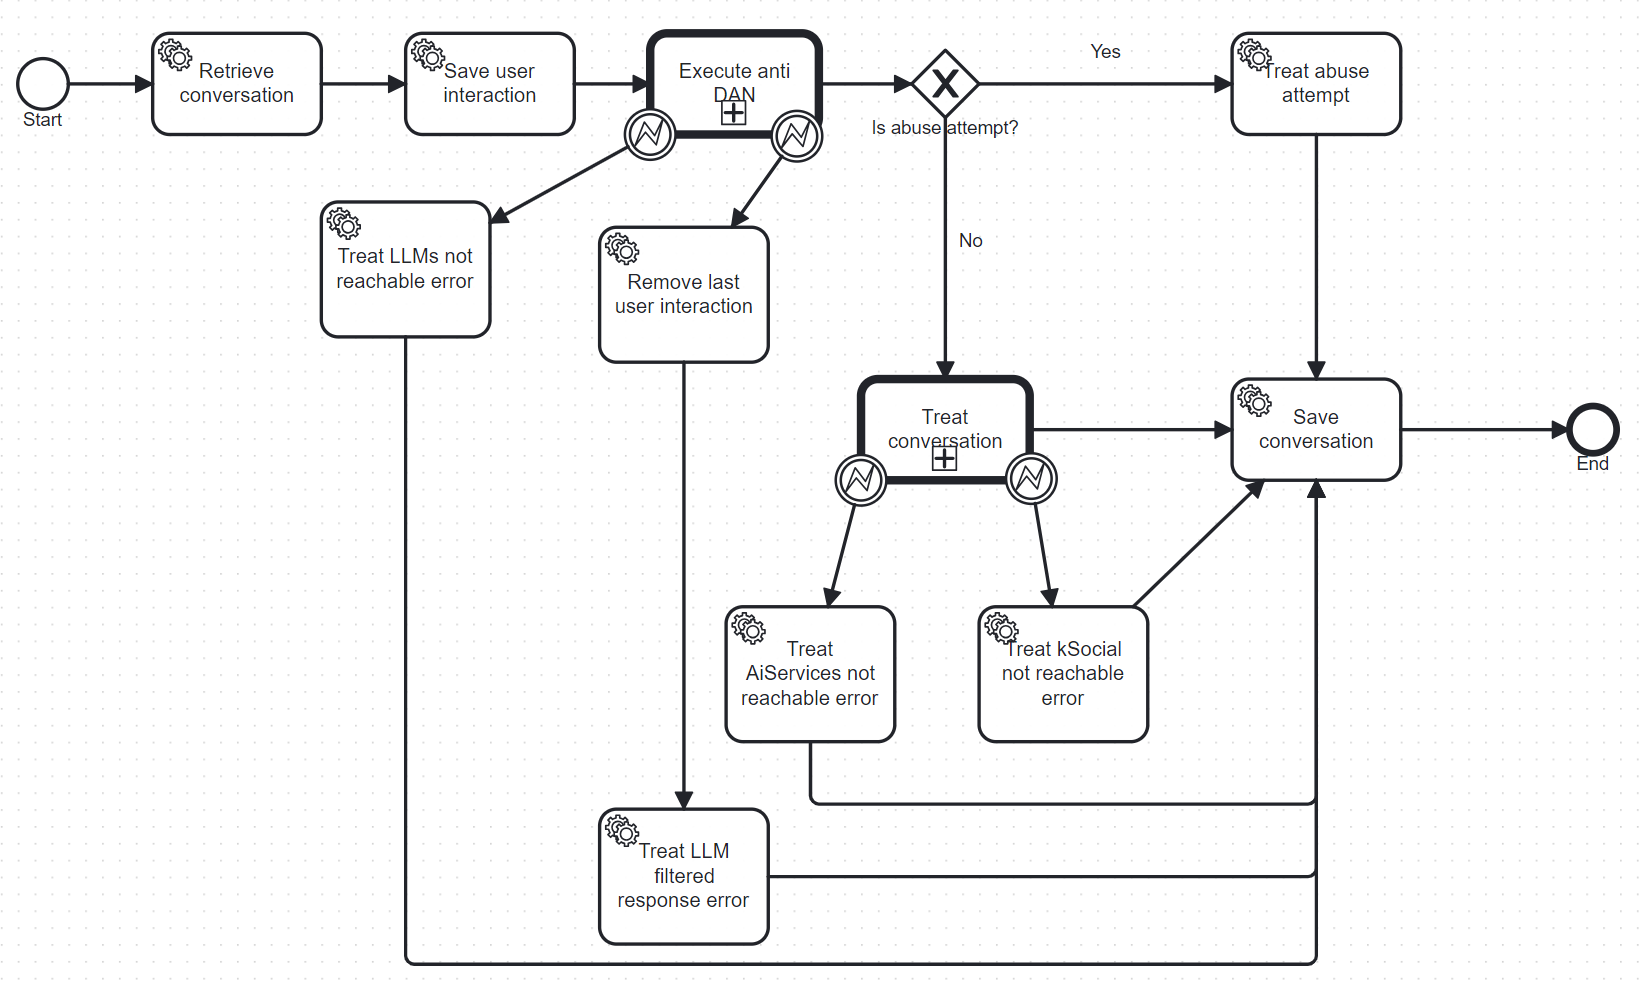
\includegraphics[width=0.7\textwidth]{img/Conversation_process.bpmn20.png}
    \caption{Diagrama de flux conversa (a alt nivell) del xatbot, en notació BPMN.}
    \label{fig:coversation_process}
\end{figure}

\section{Resultats}
\label{sec:results}

El rendiment del xatbot s'avalua mitjançant un conjunt de proves de 35 preguntes, comparant els mètodes RAG estàndard i Small to Big Retrieval (STBR). El mètode STBR demostra una precisió superior (0,79 de mitjana) en comparació amb el mètode RAG estàndard (0,65 de mitjana), amb un rendiment més consistent a través de diferents consultes. No obstant això, STBR requereix més recursos computacionals, fet que el fa adequat per a escenaris on es prioritza la precisió per sobre de la velocitat.

\begin{table}[H]
  \centering
  \begin{tabular}{|c|c|c|}
    \hline
    \textbf{Mètode}          & \textbf{Precisió \(\uparrow\)} & \textbf{Desviació Esàndar \(\downarrow\)}  \\
    \hline
    RAG Normal               & 0.65                           & 0.031                                      \\
    \textbf{RAG STBR}        & \textbf{0.79}                  & \textbf{0.024}                             \\       
    \hline
  \end{tabular}
  \caption{Resultats de l'avaluació. En negreta es mostren els millors resultats.}
  \label{tab:benchmark_results}
\end{table}

\section{Conclusions}
\label{sec:conclusions}

En el transcurs d'aquest projecte s'ha desenvolupat amb èxit un sistema de xatbot que millora la distribució d'informació sobre drets i prestacions socials als ciutadans de Catalunya. L'arquitectura modular del sistema, combinada amb models de llenguatge avançats, ofereix una solució flexible i escalable per a les necessitats de l'administració pública. L'ús de la tecnologia RAG millora significativament la precisió i la rellevància de les respostes del xatbot.

\section{Treball Futur}
\label{sec:future_work}

En un futur es podrien fer les següents millores:

\begin{itemize}
    \item \textbf{Accessibilitat Millorada:} Millorar les característiques per a usuaris amb discapacitats.
    \item \textbf{Optimització del Rendiment:} Reduir els temps de resposta i millorar l'escalabilitat.
    \item \textbf{Millora Contínua:} Proves regulars amb usuaris i desenvolupament iteratiu.
\end{itemize}

\section{Premis Patronat de la UdG}
\label{sec:awards}

El projecte presentat s'alinea directament amb la categoria ``Impuls Territorial'', ja que contribueix a incrementar la innovació i la competitivitat a les comarques gironines mitjançant l'ús de tecnologies avançades d'intel·ligència artificial aplicades a l'administració pública. La creació d'un xatbot personalitzat utilitzant models GPT i RAG no només permet millorar l'eficiència dels serveis públics, sinó que també ofereix una solució tecnològica innovadora que pot ser adaptada a altres àrees empresarials i institucionals dins del territori.

Aquest projecte millora les oportunitats del territori en diversos aspectes:

\begin{itemize}
    \item \textbf{Millora dels Serveis Públics Locals:} A través d'aquesta tecnologia, les administracions públiques de Catalunya, i per tant també les de Girona, poden optimitzar l'atenció al ciutadà, incrementant així la seva competitivitat i innovació en la prestació de serveis. Aquesta solució contribueix a la modernització digital, un aspecte clau per al desenvolupament local.
    \item \textbf{Desenvolupament Econòmic Local:} El projecte pot ser un motor d'innovació, no només per a les administracions públiques, sinó també per a altres empreses locals que poden adoptar tecnologies similars. Això fomenta la creació de noves oportunitats de negoci i impulsa l'economia de la regió.
    \item \textbf{Responsabilitat Social i Mediambiental:} En línia amb els valors de la categoria ``Impuls Territorial'', el projecte s'ha dissenyat amb una atenció especial a l'accessibilitat i la sostenibilitat. Els serveis optimitzats redueixen el temps i els recursos necessaris per a la interacció ciutadana, contribuint així a una gestió més eficient i responsable dels recursos públics.
\end{itemize}

Per tant, aquest treball exemplifica l'aprofitament de les oportunitats del territori, potenciant les interaccions entre la tecnologia desenvolupada i el desenvolupament local, amb una visió de futur que inclou responsabilitat social i mediambiental.

\end{document}
